\documentclass[aspectratio=169]{beamer}
\usepackage[utf8]{inputenc}
\usepackage{bookman}
\usetheme{Dresden}
\usepackage{graphicx}
\usepackage{hyperref}
\usepackage{todonotes}

\title[Microcontrollers]{Microcontrollers}
\author{MedTech Prototyping Skills (BME290L)}
\institute[Palmeri (Spring 2023)]{Mark L. Palmeri, M.D., Ph.D.}
\date{April 11, 2023}
\logo{
\includegraphics[width=0.1\textwidth]{BME-HorizontalLogo-Web-Blue.png}}

\begin{document}

\frame{\titlepage}

\section{Overview}
\begin{frame}{What is a microcontroller?}

    \begin{columns}
        \begin{column}{0.5\textwidth}
            \begin{itemize}
                \item An integrated circuit
                \item Not a small computer\dots more like an orchestra conductor.
            \end{itemize}
        \end{column}
        \begin{column}{0.5\textwidth}
            \centerline{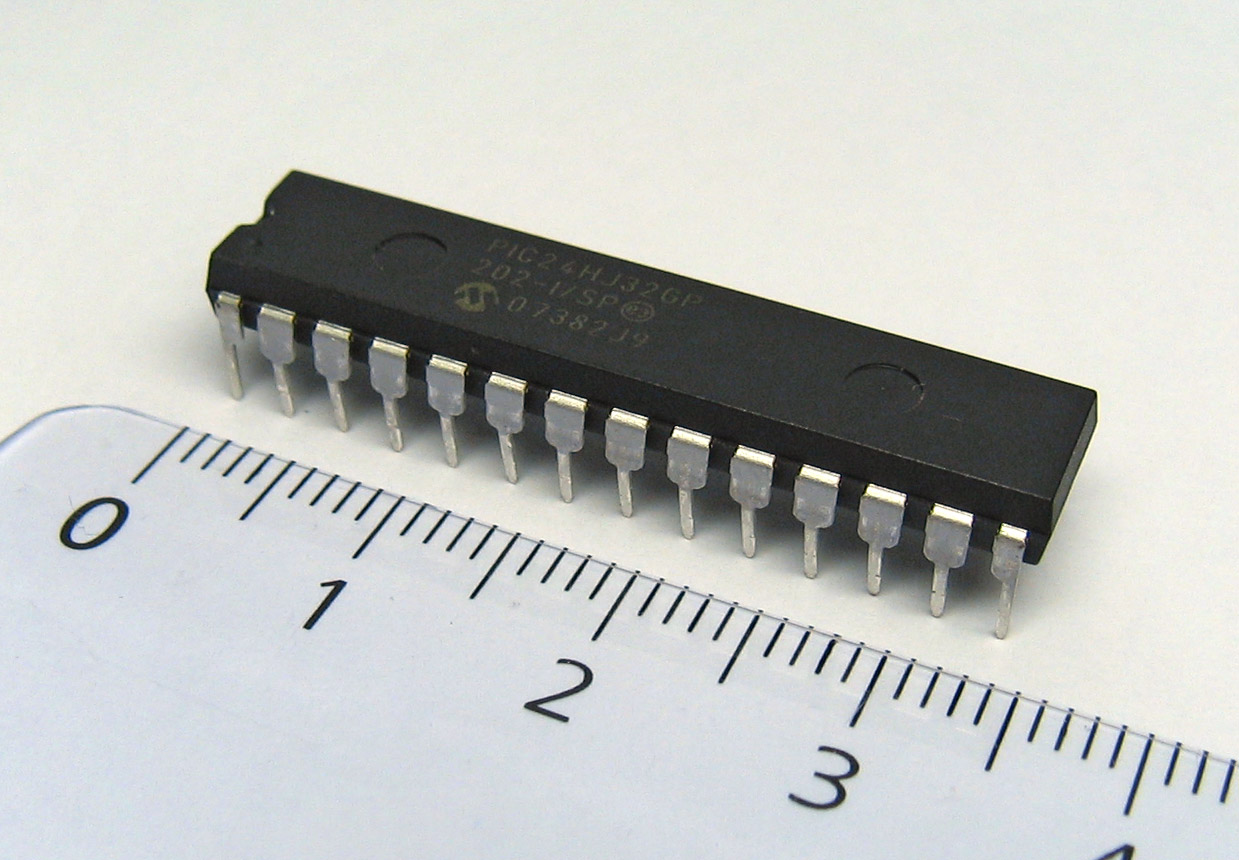
\includegraphics[width=1.0\textwidth]{ic.png}}             
        \end{column}
    \end{columns}
\end{frame}

\begin{frame}{How are microcontrollers used?}
\begin{itemize}
    \item Embedded Systems: computer systems optimized for a specific task
    \item Consumer Electronics
    \begin{itemize}
        \item Watch
        \item Remote control
        \item Music players
        \item Toys
        \item Lighting systems
    \end{itemize}
\end{itemize}

\centerline{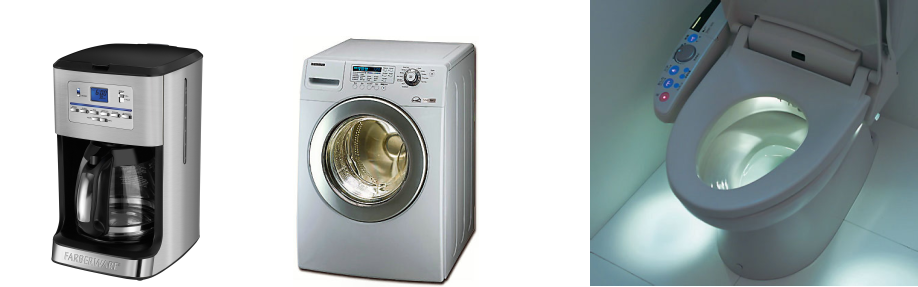
\includegraphics[width=0.5\textwidth]{consumer_electronics.png}}

\end{frame}

\begin{frame}{How are microcontrollers used?}
\begin{columns}
    \begin{column}{0.5\textwidth}
        
\begin{itemize}
    \item Civil Infrastructure
    \begin{itemize}
        \item Telecommunications
        \item Traffic Lights
    \end{itemize}
    \item Transportation
    \begin{itemize}
        \item Auto brakes, steering, radios, safety features
        \item Airplane GPS, safety features
    \end{itemize}
    \item Medical Devices
    \begin{itemize}
        \item Low power
        \item Implantable
        \item Low cost
    \end{itemize}
\end{itemize}
    \end{column}
    \begin{column}{0.5\textwidth}
       \centerline{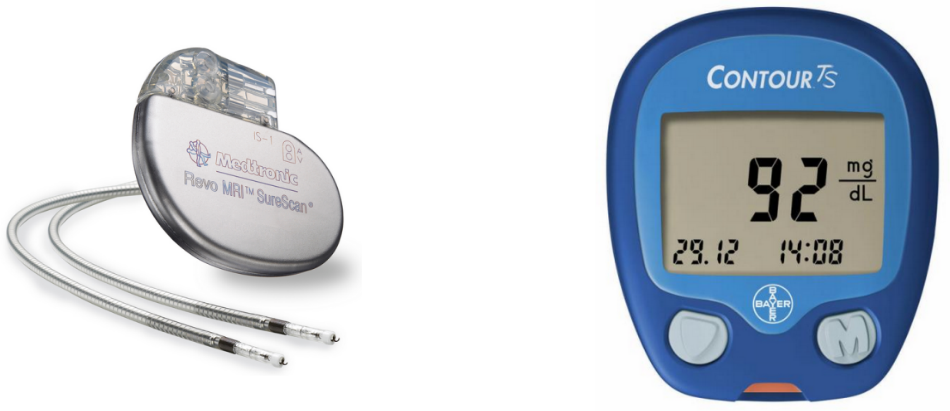
\includegraphics[width=1.0\textwidth]{medical_devices.png}} 
    \end{column}
\end{columns}

\end{frame}

\begin{frame}{Why microcontrollers?}
\begin{itemize}
    \item Large variety
    \item Can be very specialized
    \item Reprogrammable
    \item Design control systems
        \begin{itemize}
            \item Automation
            \item User input
        \end{itemize}
    \item Small physical footprint
\end{itemize}

\end{frame}

\begin{frame}{Low Power}
\begin{itemize}
    \item Low DC supply voltages
    \item Sleep current $\approxeq$ 20 nA
    \item Operating current 10-100 $\mu$A
    \item Operating Power: $\mu$W
\end{itemize}

\end{frame}

\begin{frame}{Limitations}
\begin{itemize}
    \item Very limited on-board memory ($\approx$ kB)
    \item Relatively slow (1-100 MHz)\footnote{This is changing...}
    \item Single core\footnote{This is also changing...}
\end{itemize}

\end{frame}

\section{Why Arduino?}

\begin{frame}{How do microcontrollers work?}
    Executes a program that is stored (embedded) on the microcontrollers memory.

    \begin{enumerate}
        \item Write program on your computer
        \item Compile (\textbf{build}) code into machine/assembly language that hardware can utilize
        \item \textbf{Flash} onto microcontroller (JTAG, UART,  FTDI, USB  or another interface)
        \item Bootloader begins execution of the code when the device is powered
        \item Software interacts with the hardware in the ways your code has specified
    \end{enumerate}

\end{frame}

\begin{frame}{Why Arduino?}
\begin{itemize}
    \item Great starting point
    \item Wiring (C/C++) programming interface
    \item Open-source software and hardware
    \item Standardized IO pin layout
    \item Lots of peripherals ("shields")
    \item Rapid prototyping
\end{itemize}
\end{frame}

\begin{frame}{IDE}
    \begin{columns}
        \begin{column}{0.5\textwidth}
            \begin{itemize}
                \item Simple IDE
                \item Integrated compiler ("build")
                \item Integrated firmware flashing ("upload")
            \end{itemize}
        \end{column}
        \begin{column}{0.5\textwidth}
            \centerline{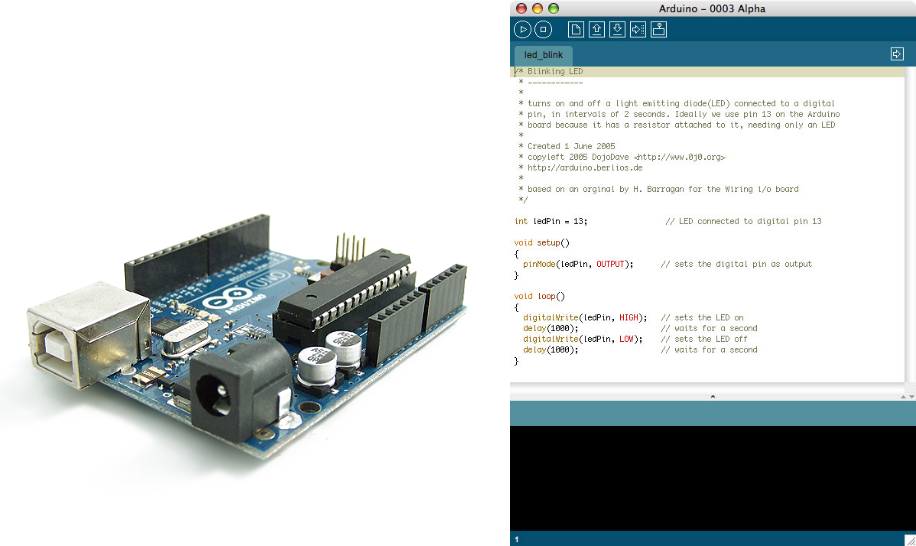
\includegraphics[width=1.0\textwidth]{ide.png}}
        \end{column}
    \end{columns}

\end{frame}

\begin{frame}{Shields}

    \centerline{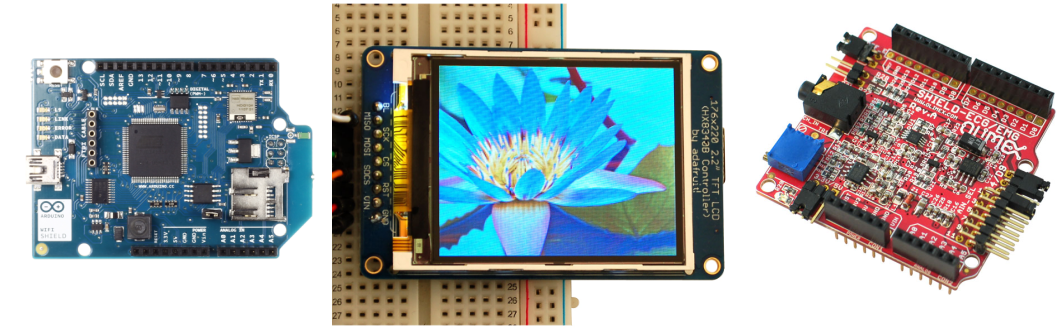
\includegraphics[width=1.0\textwidth]{shields.png}}

\end{frame}

\begin{frame}{Technical Specifications}
\begin{itemize}
    \item Logical Voltage: 1.8/3.3/5 V
    \item Frequency / Clock: \# of operations / second
    \item IO Pins
    \begin{itemize}
        \item Digital and Analog
        \item Input impedance and pull up/down voltage considerations
    \end{itemize}
\end{itemize}

\end{frame}

\begin{frame}{Development Kit}
\begin{columns}
    \begin{column}{0.5\textwidth}
        \begin{itemize}
            \item GPIO pins mapped to female headers
            \item USB $\rightarrow$ power \& flash
            \item DC barrel jack (5 V, regulated)
            \item Integrated button and LED
            \item The microcontroller is the IC; everything else is to
            facilitate connectivity and testing!
        \end{itemize} 
    \end{column}
    \begin{column}{0.5\textwidth}
        \centerline{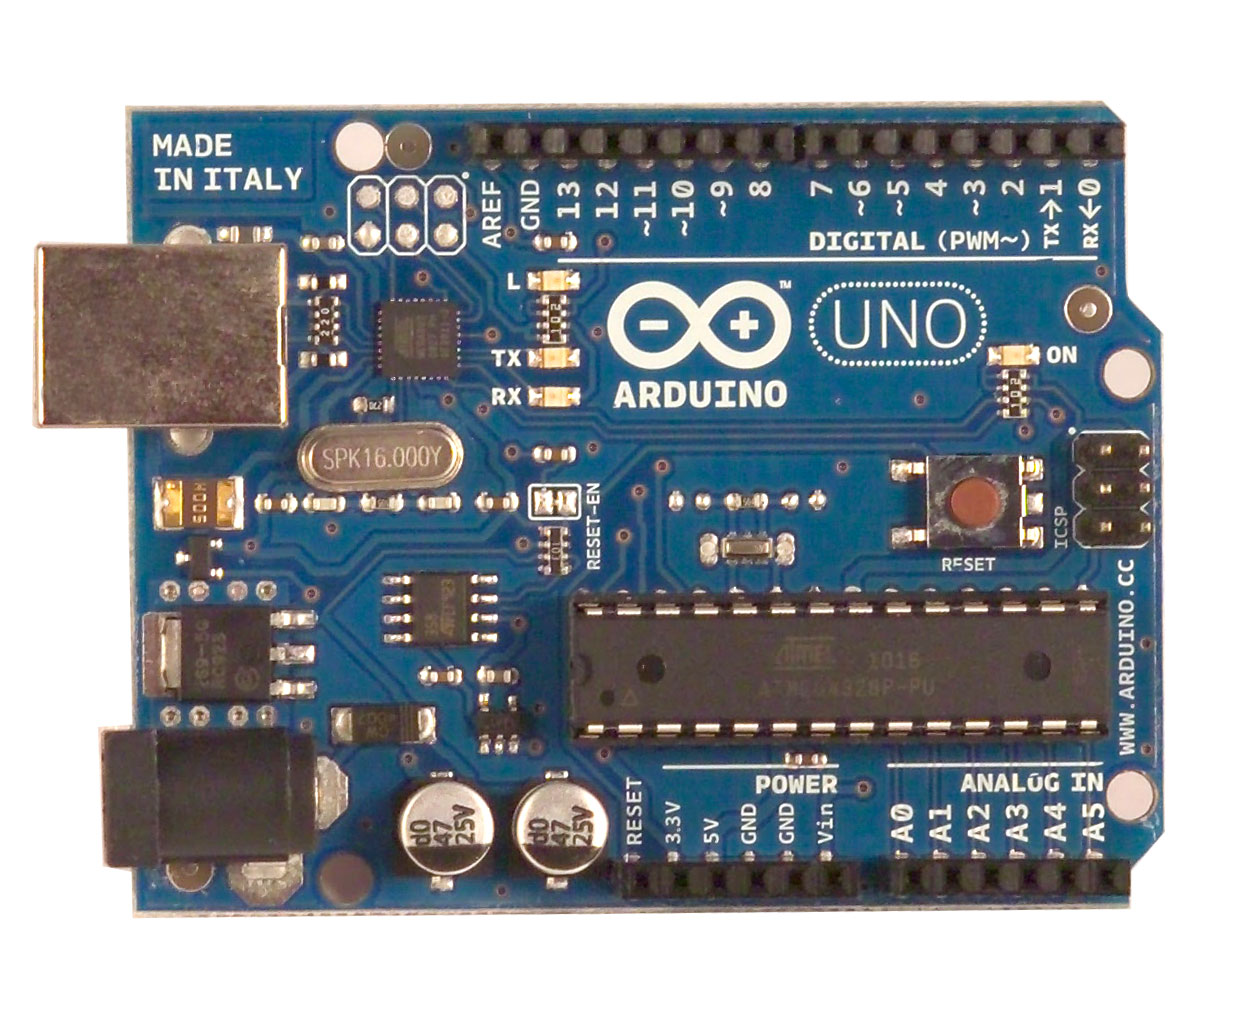
\includegraphics[width=1.0\textwidth]{arduino.png}}
    \end{column}
\end{columns}
\end{frame}

\begin{frame}{Why not Arduino?}
\begin{itemize}
    \item Actually, expensive for what it is... especially peripherals
    \item High-level abstraction of hardware control (limiting low-level control)
    \item Wiring is a non-standard language
    \item No default hardware debugger (JTAG)
    \item No unit test framework
    \item Default IDE very limiting (PlatformIO a step in the right direction)
    \item Not a Realtime Operating System (RTOS) (multithreaded), making
    timing-/priority-sensitive operations tricky.
    \item No one is getting a job based on "knowing Arduino"
\end{itemize}

\end{frame}

\section{Programming}
\begin{frame}{Types of Memory}

\begin{itemize}
    \item Flash
    \begin{itemize}
        \item Stores program and bootloader
        \item Non-volatile
    \end{itemize}
    \item EEPROM
    \begin{itemize}
        \item Stores long-term information
        \item Non-volatile
    \end{itemize}
    \item SRAM
    \begin{itemize}
        \item “RAM”
        \item Volatile
    \end{itemize}

\end{itemize}
\end{frame}


\begin{frame}{Programming a Microcontroller}
    Convert logic, algorithms, data manipulation to a form that digital hardware
    can utilize.  Common Programming Lanuages:
    
    \begin{itemize}
        \item Web dev: Javascript / PHP / HTML / Go / Python
        \item Math: Scala / Haskell / Python
        \item Databases: Ruby / PHP / SQL / MongoDB
        \item Low-Level: C / C++ / Rust
        \item Scripting: Python / Perl
        \item Mobile: Java / Dart / Objective C
        \item AI: Python / R
    \end{itemize}

\end{frame}

\begin{frame}{High Level Languages}
    \centerline{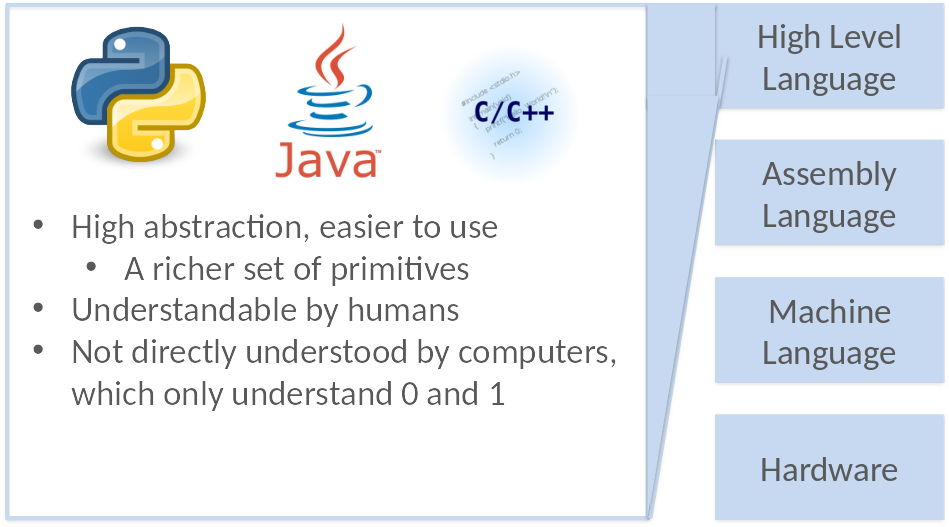
\includegraphics[width=0.7\textwidth]{high-level-langauge.png}}
\end{frame}

\begin{frame}{Assembly Languages}
    \centerline{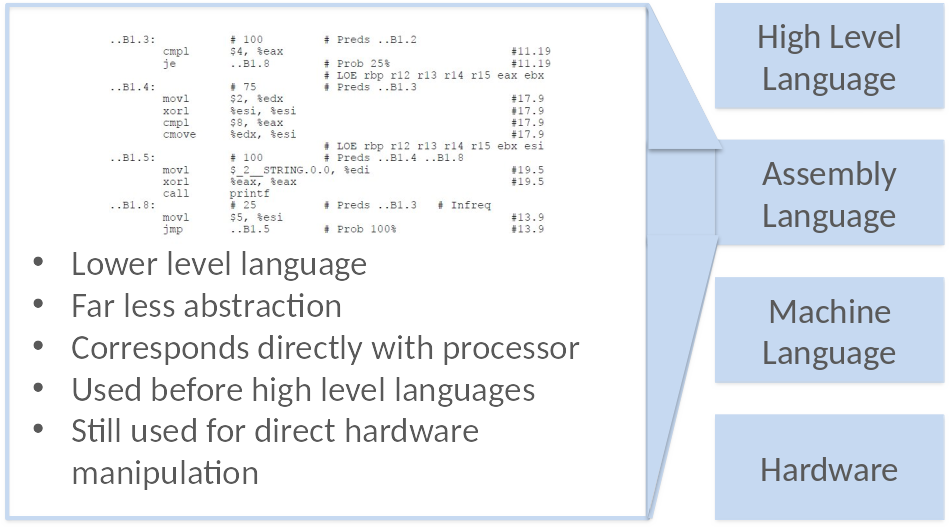
\includegraphics[width=0.7\textwidth]{assembly-language.png}}
\end{frame}

\begin{frame}{Machine Languages}
    \centerline{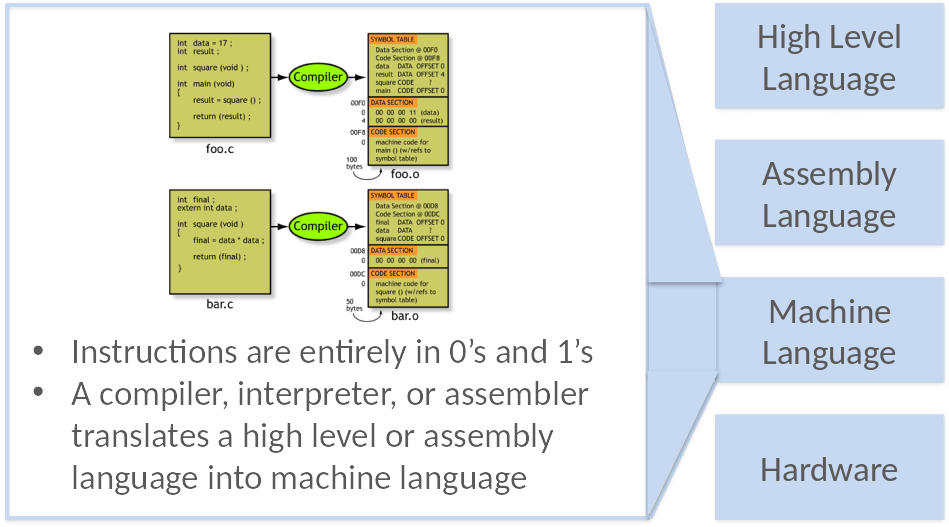
\includegraphics[width=0.7\textwidth]{machine-language.png}}
\end{frame}

\begin{frame}{Hardware Languages}
    \centerline{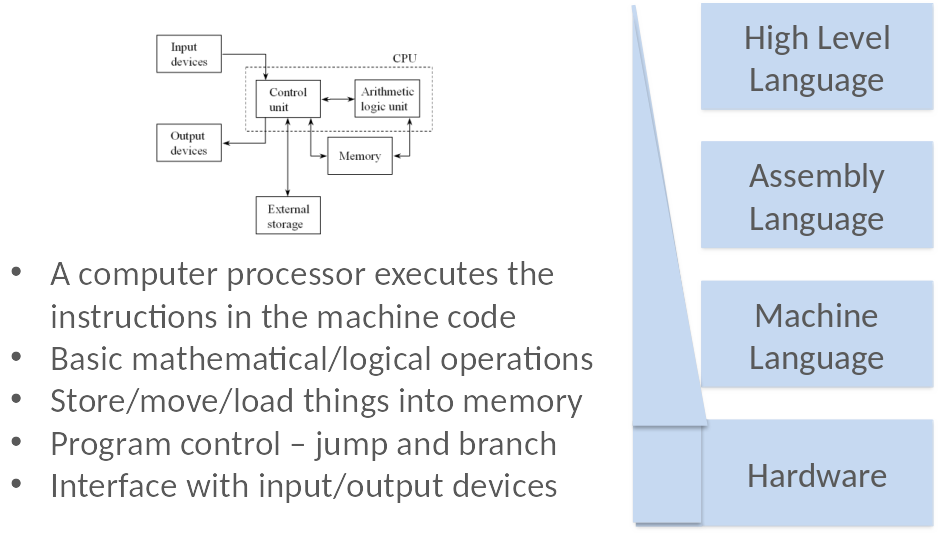
\includegraphics[width=0.7\textwidth]{hardware-language.png}}
\end{frame}

\section{Examples}

\begin{frame}{ECG}

    \centerline{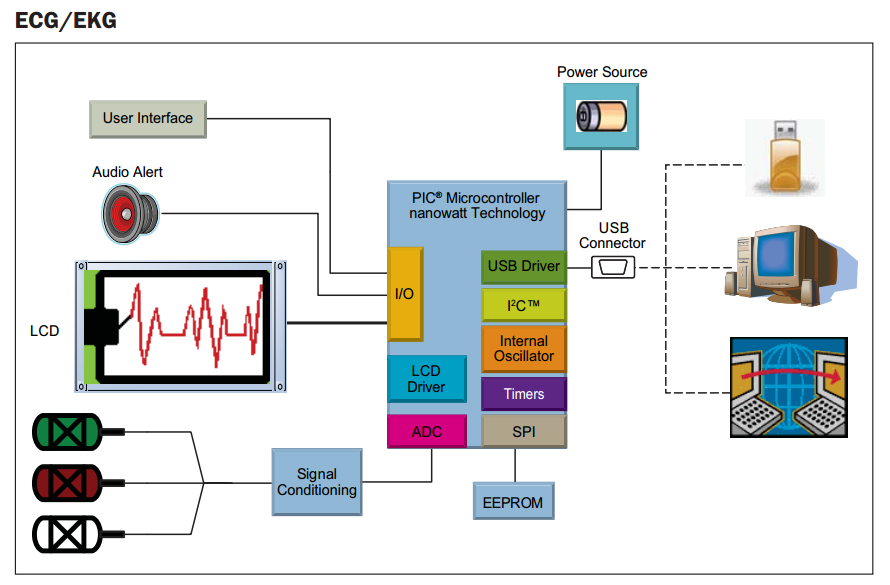
\includegraphics[width=0.6\textwidth]{ecg.png}}

\end{frame}

\begin{frame}{Pulse Oximeter}

    \centerline{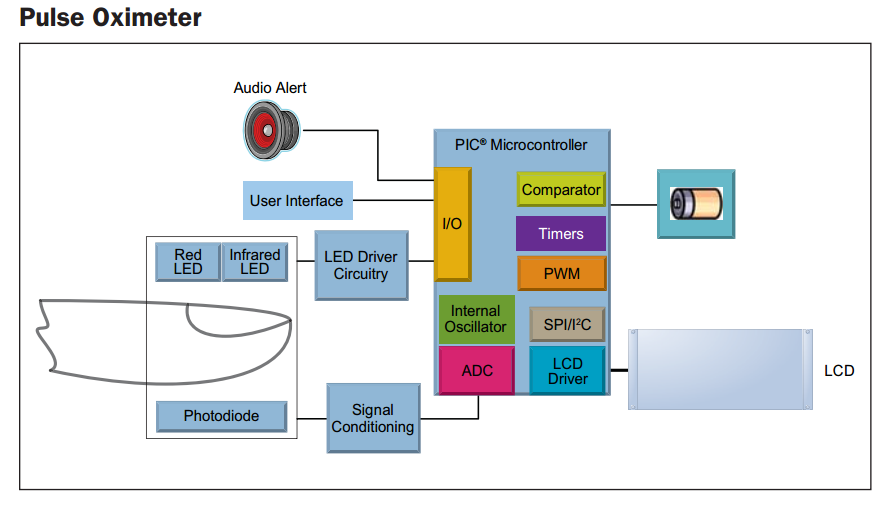
\includegraphics[width=0.7\textwidth]{pulse_ox.png}}

\end{frame}

\begin{frame}{Fun Examples}

    \begin{itemize}
        \item \href{http://vimeo.com/53476316}{Pinokio}
        \item \href{https://www.youtube.com/watch?v=Yta0aJrbOxU}{Laser Harp}
        \item \href{https://www.youtube.com/watch?v=BNBIdVR95V0}{Drink Launcher Fridge}
    \end{itemize}

\end{frame}

\begin{frame}{Function Decomposition / Block Diagram}

    Create a functional decomposition of the light enclosure device using a
    microcontroller instead of timers and logic gates.

\end{frame}

\end{document}
